\documentclass[border=5mm,tikz,preview]{standalone}
    \usetikzlibrary{arrows, arrows.meta, 
                    chains,
                    positioning,
                    shapes}
\makeatletter
\tikzset{reset join/.code={\def\tikz@after@path{}}}
\makeatother

\begin{document}
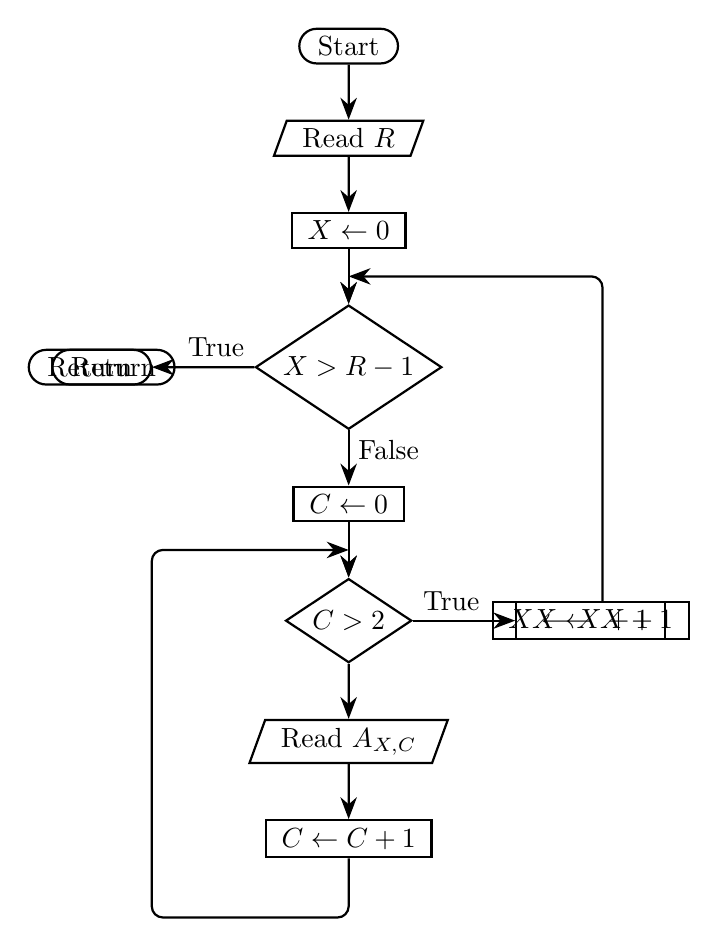
\begin{tikzpicture}[
node distance= 7mm and 13 mm,
     start chain = going below,
     base/.style = {draw, thick, align=center, 
                    inner ysep=1mm, inner xsep=2mm,
                    join=by arrow, on chain},
startstop/.style = {base, rounded rectangle},
       io/.style = {trapezium, base,
                    trapezium left angle=70, trapezium right angle=110},
  process/.style = {base},
 decision/.style = {diamond, aspect=1.5, base, inner xsep=0pt},
    arrow/.style = {-{Stealth[scale=1.2]}, rounded corners, thick}
                    ]
 % main
\node (start)   [startstop] {Start};
\node (io1)     [io]        {Read $R$};
\node (box1)    [process]   {$X \gets 0$};
\node (branch1) [decision]  {$X > R-1$};
\node (box2)    [process]   {$C \gets 0$};
\node (branch2) [decision]  {$C > 2$};
\node (io2)     [io]        {Read $A_{X,C}$};
\node (box4) [process,below=0.7 of io2] {$C \gets C+1$};
% left and right
\node (return)  [startstop,left=1 of branch1,reset join] {Return};
\node (box3)    [process, right=1 of branch2,reset join] {$X \gets X+1$};
% coordinates
\node (return)  [startstop,left=of branch1,reset join] {Return};
\node (box3)    [process, right=of branch2,reset join] {$X \gets X+1$};

\draw [arrow] (box1) -- coordinate[midway](m1)(branch1);
\draw [arrow] (box2) -- coordinate[midway](m2)(branch2);

\draw[arrow] (branch2.east) node[above right] {True} -- (box3);
%
\draw[arrow] (branch1.west) node[above left] {True} -- (return);
\node[below right] at (branch1.south) {False};
%
\draw[arrow] (box3) |- (m1);
\draw[arrow] (box4) |- + (-2.5,-1) |- (m2);
\end{tikzpicture}
\end{document}